\documentclass[11pt, letterpaper,titlepage,oneside]{article}
\usepackage{titlesec}
\usepackage{fancyhdr}
\fancyhf{}
\rfoot{\thepage}
\renewcommand{\headrulewidth}{0pt}
\pagestyle{fancy}
%paragraph indentation
\usepackage[parfill]{parskip}
\parskip = \baselineskip
\setlength{\parindent}{0in}
\usepackage{xcolor,graphicx}
\usepackage{float}
\usepackage{amsmath}
\usepackage[T1]{fontenc}
\usepackage{mathptmx}
\usepackage{lipsum}
%One and half spacing
\usepackage{setspace}
\onehalfspacing
%End one and a half spacing
\renewcommand{\arraystretch}{1}
\usepackage[margin=1in]{geometry}
% Caption Formatting
\usepackage{caption}
\captionsetup[figure]{labelsep=period}
\captionsetup[table]{labelsep=newline, justification=centering}
\renewcommand{\tablename}{TABLE}
\renewcommand{\thetable}{\Roman{table}}
\usepackage{fixltx2e}
\newcommand{\titles}{\LARGE \textbf{Literary Review}}
\newcommand{\authors}{\normalsize Tarek Ghaddar \\ Dr. Jean Ragusa}
\newcommand{\department}{\normalsize Nuclear Engineering Department}
\newcommand{\university}{\normalsize Texas A\&M University}
\newcommand{\locations}{\normalsize College Station, TX, 77843-3133}
%Script font
\usepackage[mathscr]{euscript}
\renewcommand{\thesection}{\Roman{section}.}
\renewcommand{\thesubsection}{\thesection\Alph{subsection}.}
\renewcommand{\thesubsubsection}{\thesection\Alph{subsection}.\arabic{subsubsection}}
%Include a pdf file
\usepackage{pdfpages}

\begin{document}

\begin{titlepage}
\begin{center}
  \vspace*{3.81 cm}
  \titles\\
  \vspace*{4.445cm}
  \authors \\
  \vspace*{2.54cm} 
  \department \\
  \university \\
  \locations \\
\end{center}
\end{titlepage}

\section*{The Transport Equation}

Equation \ref{transportequation} represents the discrete ordinates ($S_n$) form of the Boltzmann transport equation, where the angular flux is discretized into a set of energy groups $g$ and angular directions $m$,

\begin{equation}
\vec{\Omega}_{m}\cdot \vec\nabla \psi^{(l+1)}_{m,g} + \Sigma_{t,g}\psi_{m,g}^{(l+1)} = S_{m,g}^{(l)} + \sum_{g^\prime}\sum_{m^{\prime}}\omega_m\Sigma_{s,g^{\prime}\to g,m^\prime\to m}\psi_{m^\prime g^\prime}^{(l)}.
\label{transportequation}
\end{equation}

The left hand side of the equation represents loss terms: $\vec{\Omega}_{m}\cdot \vec\nabla$ is the leakage operator, and $\Sigma_{(t,g)}$ is the collision operator (absorption and outscatter). The right hand side represents the total source: $S_{m,g}$ represents the external source, $\Sigma_{s,g^{\prime}\to g,m^\prime\to m}$ represents the inscatter operator, and $\omega_m$ is a weighting factor for angular direction $m$. 

The preferred way to solve the $S_n$ form of the transport equation is source iteration. An initial guess is made, which occupies the right hand side of Eq. \ref{transportequation}, and the next iteration of $\psi_{m,g}$ is calculated from this. This process is repeated until $\psi_{m,g}$ converges within a user-specified tolerance. The method of solving the $S_n$ transport equation on a domain discretized in space, energy, and angle is the tranpsort sweep.

\section*{The Structured Transport Sweep}

A sweep algorithm is defined by three properties:

\begin{itemize}
\item partitioning: dividing the domain among available processors
\item aggregation: grouping cells, directions, and energy groups into tasks
\item scheduling: choosing which task to execute if more than one is available
\end{itemize}

If $M$ is the total number of angular directions, $G$ is the total number of energy groups, and $N$ is the total number of cells, then the total fine grain work units is $8MGN$. The factor of 8 is present as $M$ directions are swept for all 8 octants of the domain. The finest grain work unit is the calculation of a single direction and energy groups unknowns in a single cell, or $\psi_{m,g}$ for a single cell.

In a regular grid, we have the  number of cells in each Cartesian direction: $N_x, N_y, N_z$. These cells are aggregated into ``cellsets''. However, in an unstructured mesh, the number of cells cannot be described as such. In PDT specifically we initially subdivide the domain into subsets, which are just rectangular subdomains. Within each subset, an unstructured mesh is created. This creates a pseudo-regular grid. These subsets become the $N_x, N_y, N_z$ equivalent for an unstructured mesh. The spatial aggregation in a PDT unstructured mesh is done by aggregating subsets into cellsets. 

If $M$ is the total number of angular directions, $G$ is the total number of energy groups, and $N$ is the total number of cells, then the total fine grain work units is $8MGN$. The factor of 8 is present as $M$ directions are swept for all 8 octants of the domain. The finest grain work unit is the calculation of a single direction and energy groups unknowns in a single cell, or $\psi_{m,g}$ for a single cell.

Fine grain work units are aggregated into coarser-grained units called \textit{tasks}. A few terms are defined that describe how each variable is aggregated.

\begin{itemize}
\item $A_x = \frac{N_x}{P_x}$, where $N_x$ is the number of subsets in $x$ and $P_x$ is the number of processors in $x$
\item $A_y = \frac{N_y}{P_y}$, where $N_y$ is the number of subsets in $y$ and $P_y$ is the number of processors in $y$
\item $N_g = \frac{G}{A_g}$
\item $N_m = \frac{M}{A_m}$
\item $N_k = \frac{N_z}{P_z A_z}$
\end{itemize}

It follows that each process owns $N_k$ cell-sets (each of which is $A_z$ planes of $A_x A_y$ cells), $8N_m$ direction-sets, and $N_g$ group-sets for a total of $8N_m N_g N_k$ tasks.

One task contains $A_x A_y A_z$ cells, $A_m$ directions, and $A_g$ groups. Equivalently, a task is the computation of one cellset, one groupset, and one angleset. One task takes a stage to complete.  This is particularly important when comparing sweeps to the performance models. 

The minimum possible number of stages for given partitioning parameters $P_i$ and $A_j$ is $2 N_{\text{fill}}+N_{\text{tasks}}$. $N_{\text{fill}}$ is both the minimum number of stages before a sweepfront can reach the center-most processors and the number needed to finish a direction's sweep after the center-most processors have finished. Equations \ref{nfill}, \ref{nidle}, and \ref{ntasks} define $N_{\text{fill}}$, $N_{\text{idle}}$, and $N_{\text{tasks}}$:

\begin{equation}
N_{\text{fill}} = \frac{P_x + \delta_x}{2} - 1 + \frac{P_y + \delta_y}{2} - 1 + N_k (\frac{P_z + \delta_z}{2} - 1)
\label{nfill}
\end{equation}
\begin{equation}
N_{\text{idle}} = 2 N_{\text{fill}}
\label{nidle}
\end{equation}
\begin{equation}
N_{\text{tasks}} = 8 N_m N_g N_k
\label{ntasks}
\end{equation}
where $\delta_u$ is 1 for $P_u$ odd, and 0 for $P_u$ even.

Equation \ref{paralleleff} approximately defines parallel parallel sweep efficiency. This can be calculated for specific machinery and partitioning parameters by substituting in values calculated using Eqs \ref{nfill},\ref{nidle}, and \ref{ntasks}.

\begin{equation}
\epsilon = \frac{1}{[1+\frac{N_{\text{idle}}}{N_{\text{tasks}}}][1 + \frac{T_{\text{comm}}}{T_{\text{task}}}]}
\label{paralleleff}
\end{equation}

Equations \ref{Tcomm} and \ref{Ttask} show how $T_{\text{comm}}$ and $T_{\text{task}}$ are calculated:

\begin{equation}
T_{\text{comm}} = M_L T_{\text{latency}} + T_{\text{byte}} N_{\text{bytes}}
\label{Tcomm}
\end{equation}
\begin{equation}
T_{\text{task}} = A_x A_y A_z A_m A_g T_{\text{grind}}
\label{Ttask}
\end{equation}
where $T_{\text{latency}}$ is the message latency time, $T_{\text{byte}}$ is the additional time to send one byte of message, $N_{\text{bytes}}$ is the total number of bytes of information that a processor must communicate to its downstream neighbors at each stage, and $T_{\text{grind}}$ is the time it takes to compute a single cell, direction, and energy group.

Scheduling utilizes an algorithm to assign priority to tasks. An example of this is the ``depth-of-graph'' algorithm, which gives priority to the task that has the longest chain of dependencies. In general, a quantity $D$ is defined, which is simply the number of downstream dependents each task has. Then a simple series of logicals determines which task has priority and should be executed first:

\begin{enumerate}
\item Tasks with higher $D$ have higher priority,
\item If multiple tasks have the same $D$, then tasks with $\Omega_x > 0$ have priority,
\item The next tiebreaker is $\Omega_y > 0$,
\item The next tiebreaker is $\Omega_z > 0$,
\end{enumerate}

Another optimal scheduling algorithm (not proved) is the ``push-to-central'' algorithm. This algorithm prioritizes tasks that advance wavefronts to central planes in the processor layout. A few definitions are necessary to understand the push-to-central algorithm:

\begin{itemize}
\item $i \; \varepsilon \; (1,P_x) = $ the $x$ index into the processor array, with similar definitions for y and z indices, j and k,
\item $X = \frac{P_x + \delta_x}{2}$,
\item $Y = \frac{P_y + \delta_y}{2}$,
\item $Z = \frac{P_z + \delta_z}{2}$.
\end{itemize}

With these definitions, The push-to-central algorithm prioritizes the following tasks accordingly:

\begin{enumerate}
\item If $i \leq X$, then tasks with $\Omega_x > 0$ have priority, while for $i > X$, tasks with $\Omega_x < 0$ have priority.
\item If multiple ready tasks have the same sign on $\Omega_x$, apply rule 1 to $j,Y,\Omega_y$.
\item If multiple ready tasks have the same sign on $\Omega_x$ and $\Omega_y$, apply rul 1 to $k,Z, \Omega_z$.
\end{enumerate}

This schedule pushes tasks toward the $i = X$ central processor plane with top priority, followed by pushing toward the $j = Y$ central processor plane, followed by pushing toward the $k = Z$ central processing plane.


\section*{The Unstructured Transport Sweep}

The development of an algorithm for efficient parallel transport sweeps focuses on obtaining a good sweep ordering. This is called \textit{scheduling}. A new list scheduling algorithm has been constructed for modest levels of parallelism (up to 126 processors).

There are three requirements for a sweep scheduling algorithm to have. First, the algorithm should have low complexity, since millions of individual tasks are swept over in a typical problem. Second, the algorithm should schedule on a set of processors that is small in comparison to the number of tasks in the sweep graph. Last, the algorithm should distribute work in the spatial dimension only, so that there is no need to communicate during the calculation of the scattering source. 

Here is the pseudocode for the algorithm:

\begin{verbatim}
Assign priorities to every cell-angle pair
Place all initially ready tasks in priority queue
While (uncompleted tasks)
    For i=1,maxCellsPerStep
       Perform task at top of priority queue
       Place new on-processor tasks in queue
    Send new partition boundary data
    Receive new partition boundary data
    Place new tasks in queue 
\end{verbatim}

An important part of the algorithm above is the assigning priorities to tasks. Specialized prioritization heuristics generate partition boundary data as rapidly as possible in order to minimize the processor idle time. 

Nearly linear speedups were obtained on up to 126 processors. Further work is being done for scaling to thousands of processors. 

\subsection*{Cycle Detection}

A cycle is a loop in a directed graph. These occur commonly in unstructred meshes. The problem with cycles is that they can cause hang time in the problem, as a processor will wait for a message that might will never come. This means that the computation for one or more elements will never be completed. The solution to this is to ``break'' any cycles that exist by removing an edge of the task dependence graph (TDG). Old flux information is used on a particular element face in the domain. Most of the time, the edge removed is oriented obliquely with respect to the radiation direction. 

Algorithms for for finding cycles are called \textit{cycle detection} algorithms. This must be done efficiently in parallel, both because the task dependence graph is distributed, and because the finite element grid may be deforming every timestep and changing the associated TDG.

Cycle detection utilizes two operations: trim and mark. Trimming identifies and discards elements which are not in cycles. At the beginning of cycle detection, graphs are trimmied in the downwind direction, then the remaining graphs are trimmed in the upwind direction. A pivot vertex is then selected in each graph. Graph vertices are then marked as upwind, downwind, or unmarked. Then, if any vertices are both upwind and downwind, the cycle is these vertices plus the pivot vertex. An edge is removed between 2 cycle vertices, and 4 new graphs are created: a new cycle, the upwind vertices without the cycle, the downwind vertices without the cycle, and a set of unmarked vertices. This recursively continues until all cycles are eliminated.

\newpage

\section*{Sweep Example}

Here I will cover an example of a 2D processor layout with different aggregation factors, graphically and mathematically verifying the performance models for different partitioning parameters. It is important to note that in 2D, with $P_z$ and $A_z$ equal to 1, Eqs. \ref{nfill}, and \ref{ntasks} change slightly due to the lack of $z$ dependence. Equation \ref{updaten} shows the new expressions for $N_{\text{fill}}$ and $N_{\text{tasks}}$:
\begin{align}
N_{\text{fill}} &= \frac{P_x + \delta_x}{2} - 1 + \frac{P_y + \delta_y}{2} - 1 \\
N_{\text{tasks}} &= 4 N_m N_g\\
\label{updaten}
\end{align}
where we see that in $N_{\text{tasks}}$ we only multiply $N_m$ by 4 instead of 8, because we now deal with quadrants, not with octants.

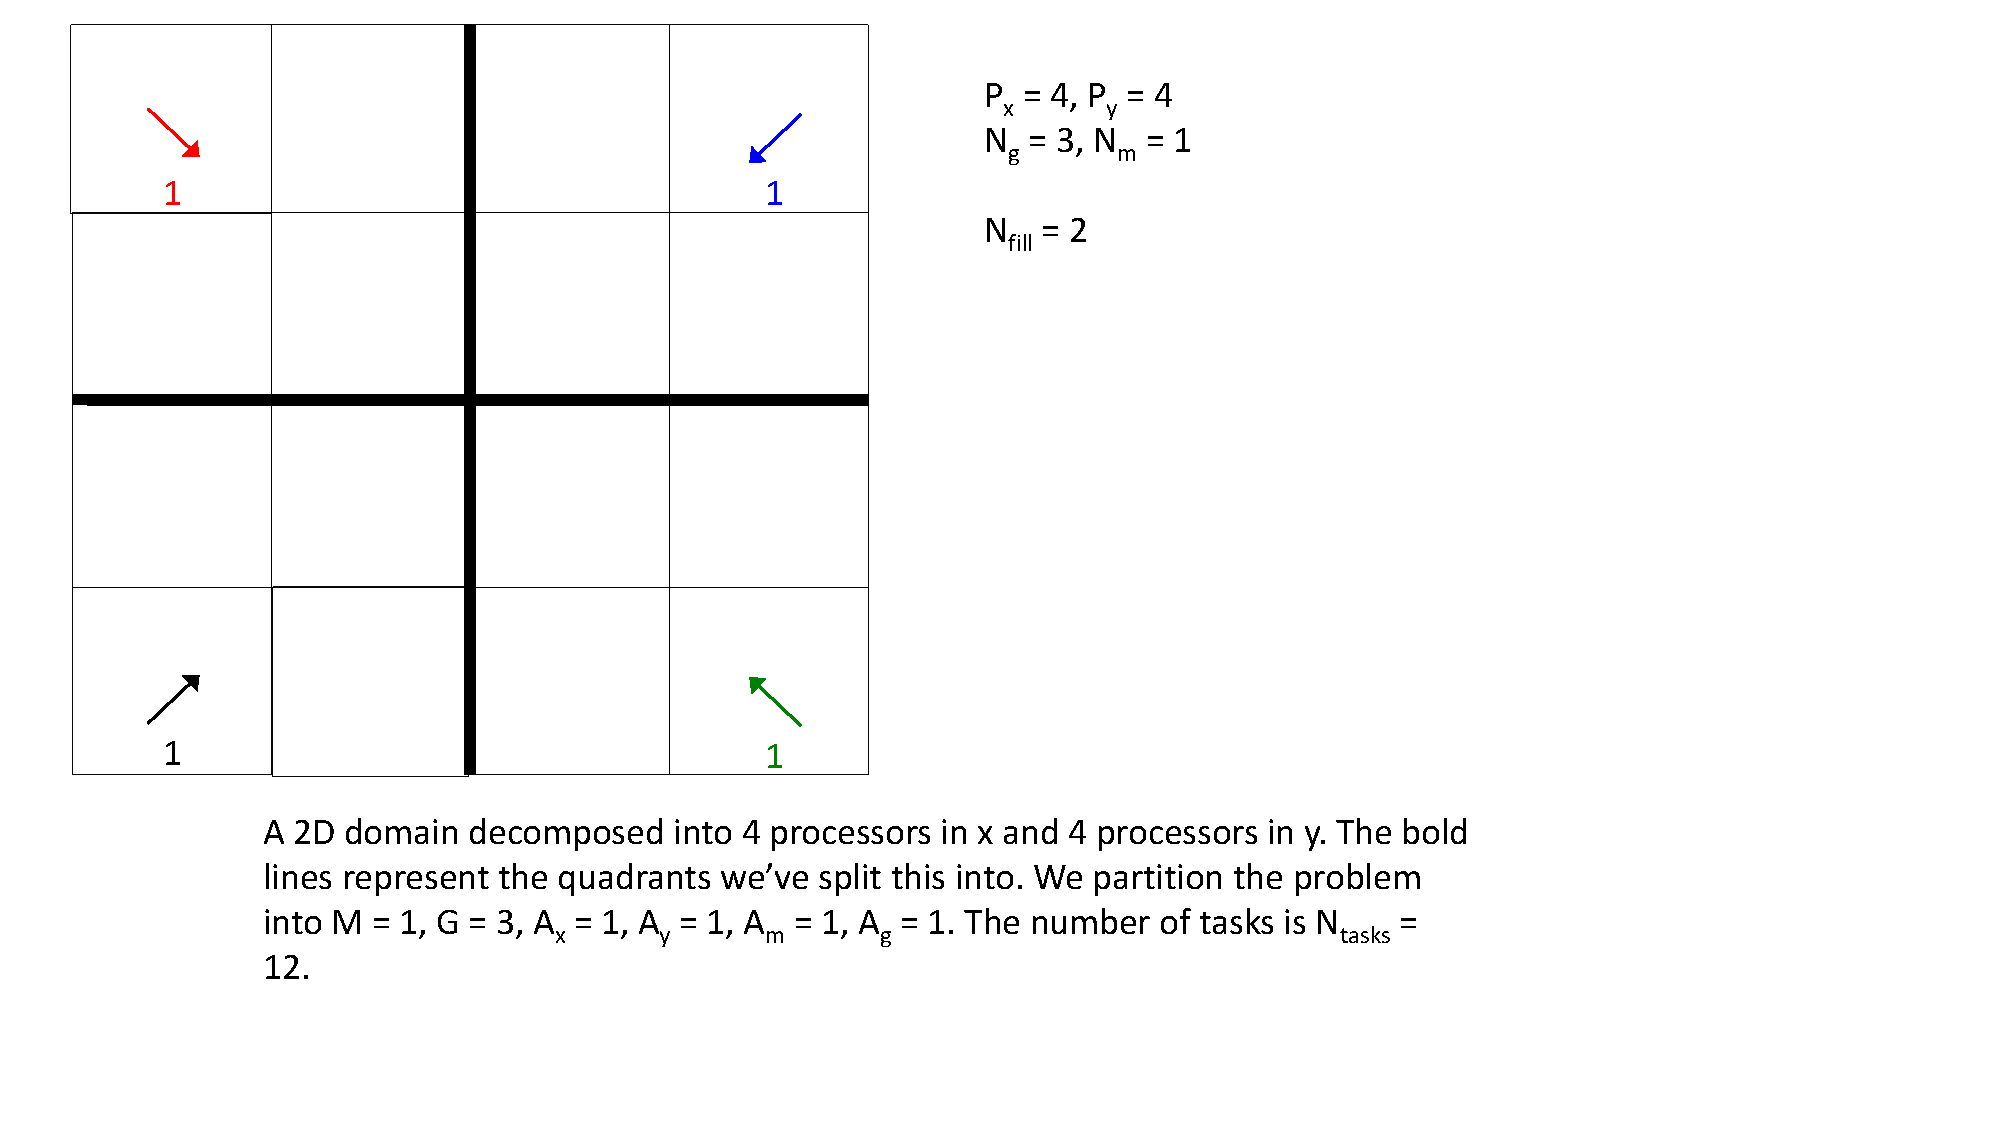
\includepdf[fitpaper,pages={1-16}]{SweepExamples.pdf}

\end{document}